%======================================================================
% 湖南科技学院本科毕业论文（设计）模板
% 编译方式：XeLaTeX；字体、版式与图表格式由 husethesis.cls / husestyle.sty 提供。
%======================================================================
\documentclass{husethesis}
\begin{document}
\pagestyle{empty}        % 封面至答辩记录表：不编页码（同原文档）

%============================ 1. 封面 =================================
% 参数：{中文题目}{英文第一行}{英文第二行}{姓名}{学号}
%       {院（系）}{专业、年级}{指导教师}{日期}
% ★ 替换为你的论文信息（标签列宽、行距、横幅尺寸等样式已内置在 husestyle.sty）
\makecover
  {基于Java的增值平台的设计与实现}
  {The Design and Implementation of}
  {Value-Added Platform Based on Java}
  {XXX}
  {201408001104}
  {信息工程学院}
  {计算机科学与技术2014级}
  {XXX（职称）、企业导师姓名（职称）}
  {2022年5月6日}

%======================== 2. 诚信声明 ==================================
% 声明正文一般无需修改；签名日期如不同，可在导言区
% \renewcommand{\integritydate}{二〇二二年\hspace{0.3em}五月\hspace{0.3em}六日}
\begin{integritystatement}
本人郑重声明：所呈交的本科毕业论文（设计），是本人在指导老师的指导下，独立进行研究工作所取得的成果，成果不存在知识产权争议，除文中已经注明引用的内容外，本论文不含任何其他个人或集体已经发表或撰写过的作品成果。对本文的研究做出重要贡献的个人和集体均已在文中以明确方式标明。本人完全意识到本声明的法律结果由本人承担。
\end{integritystatement}


%======================== 3. 目录 ======================================
\maketoc

%======================== 4. 中文摘要 ==================================
% 参数：{论文题目}{关键词（分号隔开）}；环境内为正文
%         ★ 替换为你自己的论文题目、摘要与关键词
\begin{cnabstract}{基于大数据的永州市医疗运行分析系统的设计与实现}{Java；web；预测；医疗分析}
工业4.0的到来，大数据成为这个时代的主题。随着我国网络基础信息与数字产业的发展，许多传统行业中会产生海量数据，而如何从海量数据中提取到有价值的信息，并且对这些信息进行分析，加工，传递并与传统行业相结合，显得尤为重要，而大数据的思想也在各个领域崭露头角，逐步形成以大数据为驱动融合传统行业的新趋势。

医疗是国计民生的大事，创建一个以大数据为基础的地区医疗运行分析系统，可以将这些数据进行科学的分类、存储，以这些已知的数据为基础，通过统计学，数学等建立模型将结果进行加工，最后通过饼图、柱状图、散点图等图表实现数据可视化，更好的监控并预测地区医疗发展状况与趋势。本系统采用web平台，利用MVC的设计架构与软件工程的设计思想，通过使用数据可视化展示以及加权平均法、移动平均法等计算模型，实现了动态的追踪不同时间、医疗种类、地点的医疗运行的状态，对于不同医院及地区形成针对性的决策的功能。模拟测试分析表明整个系统具备更精准、完备、个性的地区医疗运行分析功能。
\end{cnabstract}

%======================== 5. 英文摘要 =================================
% 参数：{英文题目}{Keywords（半角分号）}；环境内为正文
%         ★ 替换为你自己的英文题目、摘要与关键词
\begin{enabstract}{Design and Implementation of Yongzhou Medical Operation Analysis System Based on Big Data}{Java; web; prediction; Medical analysis}
With the advent of Industry 4.0, big Data has become the theme of this era. With the development of basic information and digital industry in China, many traditional industries will generate huge amounts of data, so it is particularly important to how to extract valuable information from the massive data, and analyze, process, transfer and integrate these information with traditional industries. And the idea of big data is also emerging in various fields, gradually forming a new trend of driving the integration of traditional industries with big data.

\begin{sloppypar}%  英文长句不自动断词，允许 Word 那样的松散行，避免溢出版心
Medical care is a major event in the national economy and people's livelihood. To create a regional medical operation analysis system based on big data, so these data can be scientifically classified and stored. We can process the results based on these known data, and established models through statistics and mathematics. And finally through the pie chart, histogram, scatter charts and other charts we can achieve data visualization, which can be better to monitor and forecast regional medical development status and trends. This system adopts a web platform and uses MVC's design architecture and software engineering design concepts to achieve dynamic tracking of medical operations at different times, medical types, and locations by using data visualization, weighted average method, and moving average method, and forms targeted decision-making function for different hospitals and regions. The simulation test analysis shows that the entire system has more accurate, complete, and individual regional medical operation analyzing capabilities.
\end{sloppypar}

\end{enabstract}

%======================================================================
%      正文部分：换用正文页边距（左右2.50cm），阿拉伯页码从 1 开始
%      （\startmainbody 内的版心上移 1.6pt、首行基线等样式已内置在 husestyle.sty）
%======================================================================
\startmainbody

%======================== 第 1 章 ======================================
\section{绪论}                     % 章标题：宋体三号加粗，形如"1 绪论"

\subsection{课题研究的背景及意义}  % 节标题：黑体四号
工业4.0的到来，大数据成为这个时代的主题。随着我国网络基础信息与数字产业的发展，在经济、工业、医疗、地理等领域每时每刻都会产生海量数据，这些数据大部分是非结构化的并且需要实时进行分析处理及保存，而现有的处理方法与平台在处理此类数据面临技术复杂度高、效率缓慢、处理不及时、数据冗余、数据丢失等痛点。而如何从海量的非结构化复杂数据中提取到隐含的内在联系及衍生的高价值信息，并且对这些信息进行分析，加工，传递并与传统行业相结合，显得尤为重要，而大数据的思想也在各个领域崭露头角，形成传统行业与大数据相结合的新模式。

医疗是关乎于社会民生的大事，而建设大数据处理系统，通过对海量数据的搜集、筛选、整理、分析，从数据中获得高价值的信息，降低数据冗余，减少因数据处理效率低引起的数据灾难、决策失误。以数据作为医疗资源分配、医疗服务均衡布局、疾控预防的核心驱动因素，形成以大数据为与医疗行业相结合便是一个突破性的创举。在经过动态调查，走访医生和患者后发现医疗资源分布不均衡，高质量医疗服务无法向下辐射。产生了“大型医院踏破门槛”、“小型医院无人可医”的现象。如何配置高水平医疗系统的辐射范围，分流病患至基层医疗机构，缓解大型医院的服务压力，提升大型医院的医疗质量，同时通过高端医疗辐射从而提升小医院的医疗质量，使得形成地区医疗平衡，降低医患纠纷。

该课题就是在这样的背景下产生，通过模拟永州市的医疗运行环境，制造出相关的模拟数据进行系统的测试与运行。可以直观的从大量数据中得到有价值的信息，同时与国家相关政策所结合，从而做到分析预警、总体规划、疾控与服务强度预测等功能，为整个地区医疗服务至医院实体做好监控与预测。

\subsection{国内外研究对比}
% 说明：模板 docx 中本节（1.2）各段的首行缩进是 21pt（Word「2 字符」按五号
%       10.5pt 折算），与其余段落的 24pt 不同；为与模板逐行一致，这里原样还原。
\setlength{\parindent}{21pt}
大数据具有五大特性，大量性、多样性、快速性、价值性与真实性，从大量的数据中快速的获得高价值的信息就成了大数据研究的课题。在早期，与医疗相关数据基本上都是纸质化的，但是随着信息行业的发展医疗数据快速的爆发，移动互联网、大数据与云计算等多种技术手段与传统医疗行业跨界结合，为医疗服务带来了更大的变化，更过的机遇。

在目前，医疗大数据有如下的应用。从使用人员的角度上来说，从管理者的角度，大数据技术可以用来大量的挖掘、分析、检测数据，从而为医疗管理系统、多层信息平台提供技术支持与数据支撑；从医生的角度，大数据技术可以向医生提供数据支持以及病情辅助决策等功能，减少医生的误判率，提高工作效率；从患者的角度，大数据技术可以支持个人医疗，对居民身体提供个性化精准的检测提醒，对患者实行疾病监控，更好的支持患者治疗。

现在国内外比较成熟的技术分布于临床辅助决策、医疗科研与健康预测三个方面。

在传统的医疗行业，医生依靠患者的信息以及自己的经验、知识对患者进行诊断治疗，导致部分决策不精准，局限性很大。通过将患者的信息、检查报告等相关医疗数据通过大数据系统做匹配，从而得到更好的、更加针对于患者的个性化治疗方案，提供给医生相关的决策支撑，使得医生更好的了解掌握病人的病情作出相应的治疗方案。

在医疗科研方面，将一段时间内的数据进行筛选、整理、分析、数据可视化，可以详细的根据不同时间、不同地点、不同人群等多种元素，结合个人、心理、社会、经济等因素研究疾病病发的特征，从而得出该种疾病的产生原因及治疗方法。

在健康监测方面，多种体感式监测设备已经广泛使用，配合每一位居民的健康档案、体检信息等为居民提供足不出户的疾病预测以及治疗方案，通过大数据技术整合这些数据，为居民提供更加个性化的健康管理方案。

\subsection{课题研究的主要内容}
\setlength{\parindent}{2\ccwd}% 恢复其余段落的 24pt 首行缩进
通过了解并发现以上地区医疗痛点，本系统主要开发一个基于web平台，利用MVC的设计模型，使用多种计算模型以及数据可视化的设计方法对本系统进行开发。实现了对已有的繁杂数据通过大数据进行分析、整理、展示，从而为使用者提供整体趋势，疾控与服务强度预测等功能，同时实现了医疗运行分析，决策支撑等功能辅助使用者更加直观的进行数据查看，提高数据分析的效率，并且利用多种计算模型使用已有数据进行预测，从而使得数据与监测预警、实时决策结合在一起，并且完成了系统与数据的管理功能。

\subsection{论文组织结构}
本文根据设计基于web平台以大数据为基础的开发，主要将论文工作分为七个章节，各章的内容具体如下：

第一章 绪论，主要是介绍了课题的开发背景及意义，课题主要开发内容与论文安排。

第二章 相关技术介绍，介绍本课题所开发系统所使用相关的技术，包含编程语言Java，python脚本，MVC框架，大数据理论等。

第三章 系统需求分析，详细介绍了整个系统功能需求及系统的可行性分析、性能分析，并且对所使用的框架技术进行了详细的描述。

第四章 系统总体介绍，详细对根据需求进行各个层面的设计，包括总体设计原则与思路、系统架构设计、系统模块划分与数据层的设计。

第五章 系统功能实现，详细的介绍了本系统总体框架及口设计，描述了各个功能模块的实现。

第六章 系统测试，对系统进行逻辑，性能等多方面的测试，来保证系统的安全性、流畅性等。

第七章 总结与展望，总结开发过程中遇到的问题与解决方法，考虑系统拓展性，并对可提高的地方作描述。

\subsection{本章小结}
通过本章节的描述，阐述了将大数据与医疗相结合研究的背景与意义，明确了本次课题研究的主要内容，对整体研究内容进行了初步的说明，对国内外的研究作了相关的了解，同时规划了论文的整体架构和章节划分。
\clearpage                        % 每章另起一页

%======================== 第 2 章 ======================================

\section{相关技术简介}


\subsection{Java简介}
Java隶属于SUN公司，于2009年SUN公司被甲骨文收购。前身Oak语言，由于1995年互联网的蓬勃发展给了Oak机会，由于它是按照嵌入式系统硬件平台体系结构进行编写的，所以非常小，特别适用于网络上的传输系统，而Oak也是一种精简的语言，程序非常小，适合在网络上传输[1]。Sun公司首先推出了可以嵌入网页并且可以随同网页在网络上传输的Applet（Applet是一种将小程序嵌入到网页中进行执行的技术）。在申请注册商标时，发现Oak已经被人使用了，再想了一系列名字之后，最终，使用了提议者在喝一杯Java咖啡时无意提到的Java词语，并将Oak更名为Java。1996年1月，SUN公司发布了Java的第一个开发工具包JDK 1.0。1997年2月Sun公司在Java One开发者大会上宣布开放Java核心源代码，以鼓励更多的人参与到Java社团活动中。

Java是一门面向对象编程语言，不仅吸收了C++语言的各种优点，还去掉C++中难以理解的多继承指针等概念。具有简单性、面向对象、分布式、健壮性、安全性、平台独立与可移植性、多线程、动态性等特点。由Java编程语言，JAVA类文件格式，Java虚拟机，Java应用程序接口四个部分组成[2]。

\subsection{框架简介}

\subsubsection{SSM简介}
Spring是一个轻量级的Java框架兴起于2003年，由Rod Johnson在其著作Expert One-On-One J2EE Development and Design中阐述的部分理念和原型衍生而来。SSM框架由Spring、springMVC、MyBatis三个开源框架整合而成，是现在主流的Web项目框架。它是为解决企业应用开发太过于复杂而被创建的，Spring只使用基本的JavaBean可以完成以前许多只能由EJB（JavaEE服务端组件模型）完成的事情[3]。Spring的用途不仅仅服务端的开发，从简单性、可测试性和松耦合的角度而言，基本上任何Java应用都可以从Spring中受益。

Spring的两个主要的核心面向切面（AOP）和控制反转（IoC）。Spring MVC属于SpringFrameWork的后续产品，已经融合在Spring Web Flow里面[4]。Spring MVC分离了控制器、模型对象、分派器以及处理程序对象的角色，这种分离让它们更容易进行定制，SpringMVC2.5版本以后增加了新的特点支持注解让开发人员使用起来更加方便。SpringMVC和struts相比主要的不同点在于控制视图和模型的交互机制不同，并且可以和Spring无缝链接，虽然Struts也可以实现无缝链接，但是过程会比较麻烦。Struts是Action级别而SpringMVC是方法级别更容易实现RESTful风格,而且SPringMVC比Struts更加易懂可以将更多的时间投入到实际应用当中[5]。

MyBatis是一个基于Java的半自动持久层框架，本来是apache的一个开源项目名为iBatis，2010年这个项目由apache software foundation迁移到了google code，并且改名为MyBatis。2013年11月迁移到Github。它支持SQL查询，存储过程和高级映射。MyBatis消除了几乎所有的JDBC代码和参数的手工设置以及结果集的检索。MyBatis使用简单的XML或注解用于配置和原始映射，将接口和Java的POJO（s Plain Ordinary Java Objects，普通的Java对象）映射成数据库中的记录。MyBatis和Hibernate相比更加容易掌握可以将更多的时间投入到实际应用当中。虽然Mybatis易于掌握灵活度高，但是无法做到和数据库无关系，如果需要支持多种数据库需要写多套sql映像文件工作量[6]。Mybatis工作流程如图2-1所示。

% ---- 插图：图居中，题注"图X-X 名称"，宋体五号居中 ----
% 使用从原 DOCX 中提取的图片 fig2-1_springmvc.png（原图宽约14.6cm）；
% 替换为自己的图片时，只需更换文件名与宽度即可。
\begin{figure}[htbp]
  \centering
  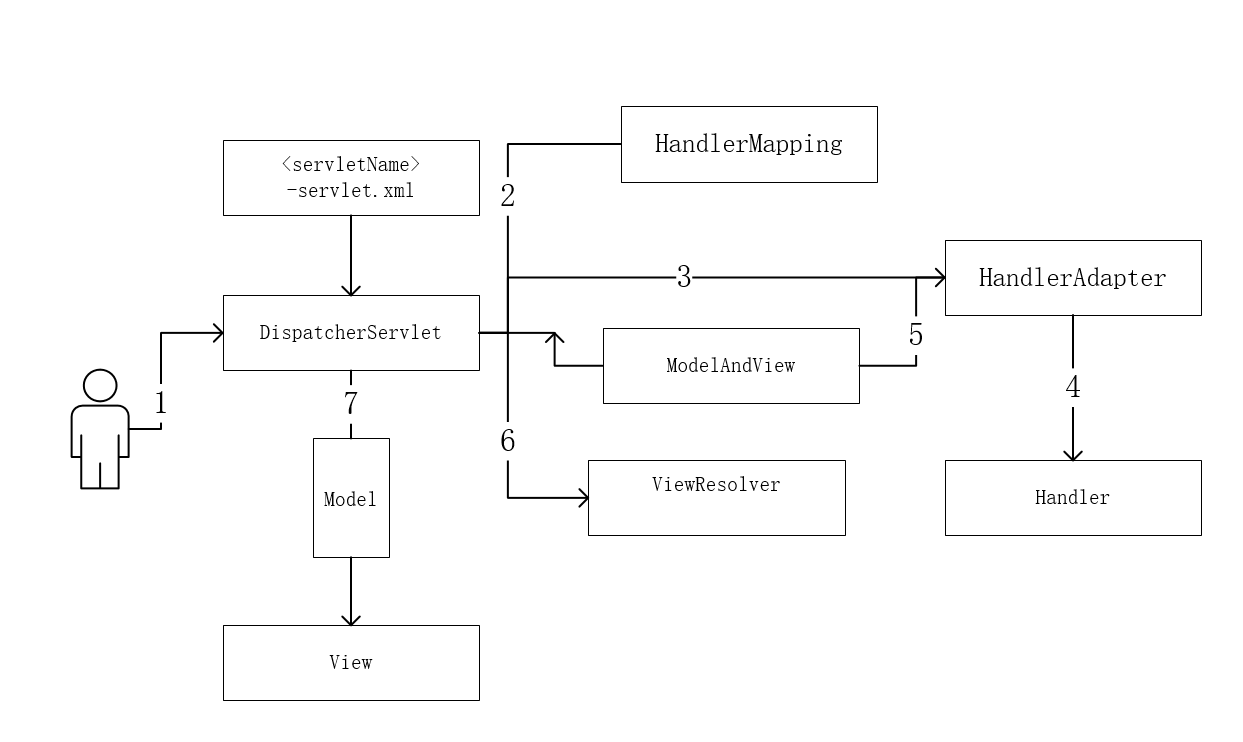
\includegraphics[width=14.6cm]{figures/fig2-1_springmvc.png}
  \caption{SpringMVC实现原理}
  \label{fig:2-1}
\end{figure}

\subsubsection{AngluarJS简介}
AngluarJS诞生于2009年，由Misko Hevery等人创建，后为Google所收购。是一款优秀的前端JS框架，已经被用于Google的多款产品当中。AngularJS有着诸多特性，最为核心的是：MVW（Model-View-Whatever）、模块化、自动化双向数据绑定、语义化标签、依赖注入等等[7]。AngluarJS为了克服HTML在构建应用上的不足而设计的，主要合适构建CRUD应用，为开发人员呈现更高层次的抽象来简化应用开发。

AngluarJS和JQuery相比：JQueryJS通过显示操作DOM来创建应用程序适合回合式应用，而AngluarJS将游览器吸收为应用程序的基础适合单页应用，减少向后端请求的数据量，减少带宽提示Web应用的性能。随着现代Web应用的高速发展Web开发模式慢慢向单页应用转移，不仅时初始过程得到了优化，也在开发复杂度较高的大型应用上，结合MVC思想，体现了其强大的优势。

\subsection{MVC简介}
Spring是一个轻量级的Java框架兴起于2003年……

\subsection{本章小结}
本章主要对该系统开发所使用的语言、后端使用的框架、所使用的数据库和使用的开发模式做了简单的介绍。采用了对比的形式对比其他框架，解释为什么使用该框架而不是其他框架。为系统的后续开发奠定了坚实的理论基础。
\clearpage

%======================== 第 3 章 ======================================

\section{系统需求分析}


\subsection{总体定位与建设目标}
Spring是一个轻量级的Java框架兴起于2003年Spring是一个轻量级的Java框架兴起于2003年Spring是一个轻量级的Java框架兴起于2003年Spring是一个轻量级的Java框架兴起于2003年……

\subsection{功能需求分析}
Spring是一个轻量级的Java框架兴起于2003年……

\subsubsection{数据采集入库功能}
AngluarJS诞生于2009年，由Misko Hevery等人创建，后为Google所收购。是一款优秀的前端JS框架。

\subsubsection{数据分析展示功能}
AngluarJS诞生于2009年，由Misko Hevery等人创建，后为Google所收购。是一款优秀的前端JS框架。

\subsubsection{系统决策支持功能}
AngluarJS诞生于2009年，由Misko Hevery等人创建，后为Google所收购。是一款优秀的前端JS框架。

\subsubsection{系统管理功能}
AngluarJS诞生于2009年，由Misko Hevery等人创建，后为Google所收购。是一款优秀的前端JS框架。

\subsection{可行性分析}
Spring是一个轻量级的Java框架兴起于2003年……

\subsubsection{经济可行性分析}
AngluarJS诞生于2009年，由Misko Hevery等人创建，后为Google所收购。是一款优秀的前端JS框架。

\subsubsection{技术可行性分析}
AngluarJS诞生于2009年，由Misko Hevery等人创建，后为Google所收购。是一款优秀的前端JS框架。

\subsection{性能分析}
Spring是一个轻量级的Java框架兴起于2003年。AngluarJS诞生于2009年，由Misko Hevery等人创建，后为Google所收购。是一款优秀的前端JS框架。

\subsection{本章小结}
AngluarJS诞生于2009年，由Misko Hevery等人创建，后为Google所收购。是一款优秀的前端JS框架。
\clearpage

%======================== 第 4 章（含三线表示例）=======================

\section{系统总体设计}


\subsection{总体设计原则及方法}
（1）整体规划设计

系统从整体进行规划设计，由顶层向各个一级、二级功能成金字塔式进行设计，从数据收集，分析，展示，预测等四个方面进行分层设计，以实现功能协调、系统健壮、结构统一、系统标准化的效果，优化系统设计思路，完善软件设计方法，提高系统容错率，避免出现因设计不规范导致的系统奔溃，重复开发等问题。

（2）结构灵活、设计规范

系统采取科学的构建模式，采取面向对象的设计方法，在开发过程中遵守高内聚低耦合的设计原则，使程序更加结构化、模块化，在后期开发过程中增强代码可读性、复用性。在补充开发的过程中可以很好地嵌入已有系统，实现只提供接口，不展示具体逻辑，可以与其他接口进行功能吻合。

\subsection{系统架构设计}

\subsubsection{视图控制层}
视图控制层主要负责分析过后数据的展示以及用户与系统交互功能。通过keshiduibi-View-browser, yiliaoduibi-View-browser, jikongfenxi-View-browser等系统交互展示页面组成。其主要展示数据分析，决策支撑，数据基础功能，系统管理等四个一级页面及其下属页面，同时负责这些页面的用户交互功能。

\subsubsection{业务逻辑层}
AngluarJS诞生于2009年，由Misko Hevery等人创建，后为Google所收购。是一款优秀的前端JS框架。

\subsection{系统模块划分}
AngluarJS诞生于2009年，由Misko Hevery等人创建，后为Google所收购。是一款优秀的前端JS框架。

\subsubsection{总体功能}
AngluarJS诞生于2009年，由Misko Hevery等人创建，后为Google所收购。是一款优秀的前端JS框架。

\subsubsection{数据分析展示模块}
AngluarJS诞生于2009年，由Misko Hevery等人创建，后为Google所收购。是一款优秀的前端JS框架。

\subsection{系统数据层设计}
数据库物理设计阶段主要任务是根据微生活的具体特征，为己给定的数据库模型选择比较合适的存储结构与存取方式。以下主要对数据库表的详细设计进行说明。

（1）T\_AGENT\_DICT 字典表，用于储存网页中下拉列表字段，当需要更改下拉列表时候不需要更改代码，可在相应的页面修改，具体结构表4-1所示。

% ---- 三线表示例（原文"表格部分有修改"即正文表格采用三线表）----
% 题注在表上方："表X-X 名称"，宋体五号居中；表内文字五号
\begin{table}[htbp]
  \centering
  \caption{字典表}
  \label{tab:4-1}
  \zihao{5}
  \begin{tabular}{llll}
    \toprule
    名字 & 类型 & 约束 & 注释 \\
    \midrule
    ID & NUMBER(10) & 非空 & ID号 \\
    PARENT\_ID & VARCHAR2(64) &  & 上级ID号 \\
    CODE & VARCHAR2(255) &  & 代码 \\
    NAME & VARCHAR2(255) &  & 名称 \\
    SEQ & NUMBER(3) &  &  \\
    TYPE & VARCHAR2(255) &  &  \\
    IS\_CATAGORY & VARCHAR2(3) &  & 是否目录 \\
    IS\_DELETE & NUMBER(3) & 默认‘0’ &  \\
    CREATE\_TIME & TIMESTAMP(6) &  &  \\
    CREATE\_BY & VARCHAR2(64) &  &  \\
    UPDATE\_TIME & TIMESTAMP(6) &  &  \\
    UPDATE\_BY & VARCHAR2(64) &  &  \\
    REMARK & VARCHAR2(100) &  &  \\
    \bottomrule
  \end{tabular}
\end{table}

（2）T\_AGENT\_LOGIN\_LOG 登录日志信息表，用于储存登陆的日志信息，包括登陆IP，账号，密码，时间等……

\subsection{本章小结}
通过本章的描述，从总体、功能、数据三个方面进行设计说明。阐述了本系统的总体设计原则与方法，对系统整体架构作出设计，对需求提出的功能进行相应的模块划分与开发设计，对数据层进行相应的设计，为系统开发提供了总纲。
\clearpage

%======================== 第 5 章 ======================================

\section{系统功能的实现}


本节主要描述需求中各功能设计的实现思路及方法，以下将分为数据分析展示，决策支持，系统基础功能，系统管理功能四个方面进行描述。

\subsection{数据分析展示}
本一级模块主要负责数据的提取，分析，并在前台进行可视化展示。其下包括地区对比、科室对比、疾控分析、政策预见四个二级模块。

\subsubsection{地区对比模块}
系统通过读取diquduibi.xml文件，在页面上生成相应的展示界面，通过diquduibi.java类进行后台控制。整个页面分为三部分，标题与月份选择为第一部分，chart与tabSheet为第二部分，报表数据为第三部分，如图5-1所示。

% ---- 图5-1：原 DOCX 中的 EMF 流程图已转换为 PNG（fig5-1_diquduibi.png）----
\begin{figure}[htbp]
  \centering
  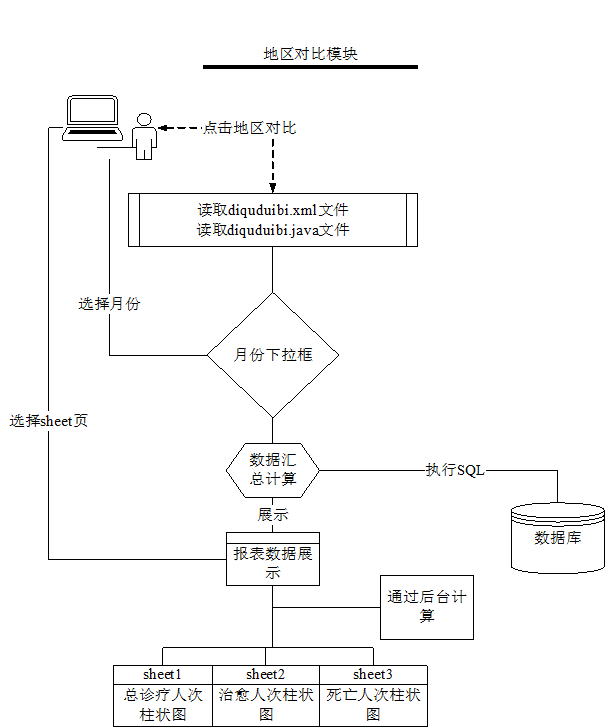
\includegraphics[width=11cm]{figures/fig5-1_diquduibi.png}
  \caption{地区对比模块流程图}
  \label{fig:5-1}
\end{figure}

\subsubsection{科室对比模块}
系统通过读取相应的keshiduibi.xml文件进行页面的设计与规划。通过keshiduibi.java进行后台行为的控制。

\subsection{决策支撑}

\subsubsection{医疗强度预测模块}
系统通过读取相应的keshiduibi.xml文件进行页面的设计与规划。通过keshiduibi.java进行后台行为的控制。

\subsubsection{疫情预警预测模块}
系统通过读取相应的keshiduibi.xml文件进行页面的设计与规划。通过keshiduibi.java进行后台行为的控制。

\subsection{本章小结}
通过本章的描述，详细的从数据分析展示、数据预测、系统数据与功能管理三个方面如何实现进行介绍。对功能实现以流程图进行展示，并辅以文字说明进行阐述，对总体设计中提出的设计进行实现。
\clearpage

%======================== 第 6 章 ======================================

\section{测试}


软件工程的测试包括技术方向的测试以及工程方向的测试两部分，通过对于软件产品这两部分的测试，尽量多的发现测试过程中所出现的软件缺陷，降低软件在上线以后出现常识性错误以及影响整个系统运行的错误。

\subsection{常用测试方法}
从软件架构方面主要分为以下三种测试方法：

（1）黑盒测试

黑盒测试也被称作功能测试，通过需求说明书进行输入值与输出值，UI交互功能的使用来进行测试，通过测试系统是否可以输出正确信息，UI交互功能是否可以达到预期的效果。

（2）白盒测试

白盒测试也被称为逻辑测试，通过需求审查与代码审查，结合需求功能设计进行系统内部的代码逻。

\subsection{测试结果}
本系统通过使用上述测试方法，分别对数据采集，数据分析展示，数据预测预警，系统管理等四个方面进行测试。

\subsection{本章小结}
通过对本章的描述，对系统进行多层次，多方法的测试。通过对数据采集、数据分析展示、数据预测预警、管理功能等模块进行黑盒、白盒测试，同时将测试结果以展示图与表格形式展示，对整个系统运行效果进行测试。
\clearpage

%======================== 第 7 章 ======================================

\section{总结与展望}


\subsection{全文工作总结}
本文设计并实现了基于大数据的永州市医疗运行分析系统，是大数据与传统行业相结合，展露新头角的一种尝试。基于大数据的永州市医疗运行分析系统的设计与实现，对于未来探索数据驱动传统行业起的了一定的帮助。本文对大数据分析系统的开发与设计的总结包括以下三点：

\subsection{对未来的展望}
（1）本系统所统计的数据因涉及保密所以为模拟数据。数据可视化页面展示的类型和数据展示的种类偏少；对于整个数据收集工作还没有做到位；在预测算法中只选择了两种预测算法；同时系统中数据种类偏少，可以作为一个数据与医疗相结合的样板，却不能成为一个真正完美的大数据分析系统。

在下一步的设计中，将会融入更多的数据类型，使用多种预测算法，对数据进行更加精确的分析预测。

（2）在整个系统中，体现了数据预处理、数据可视化与数据预测，在初步规模上已有大数据分析的雏形。
\clearpage

%======================== 参考文献 =====================================
% 版式（模板提示）："参考文献"四号黑体居中、不加粗、固定行距20磅、段前段后0，后面空一行；
%         条目小四宋体、固定行距20磅、段前段后0；编号后空一格；
%         转行时与上行作者名首字对齐（悬挂缩进）；半角标点后跟一个空格。
%         补充说明：参考文献要求 20 篇左右，按 GB/T 7714 著录，此处沿用原文示例。
%         ★ 请补充至 20 篇左右，并删除条目末尾的"（XX格式）"字样
\begin{references}
\bibitem{ref1} Vu K, Zheng R, Gao J. Efficient algorithms for k-anonymous location privacy in participatory sensing[C]//Proceedings of the IEEE International Conference on Computer Communications (INFOCOM). IEEE, 2012: 2399-2407.(国际会议格式)

\bibitem{ref2} 赵婧, 张渊, 李兴华, 等. 基于轨迹频率抑制的轨迹隐私保护方法[J]. 计算机学报, 2014, 37(10): 2096-2106. (中文期刊格式)

\bibitem{ref3} Zhang Y, Tong W, Zhong S. On Designing Satisfaction-Ratio-Aware Truthful Incentive Mechanisms for k-Anonymity Location Privacy[J]. IEEE Transactions on Information Forensics and Security, 2016, 11(11): 2528-2541. (英文期刊格式)

\bibitem{ref4} 卢卫. 2015中国互联网产业综述与2016发展趋势报告[R]. 北京：中国互联网协会, 2016. http://www.isc.org.cn/zxzx/xhdt/listinfo-33050.html.(互联网报道格式)

\bibitem{ref5} 胡秀娟. 大数据时代新闻可视化的媒介环境学研究[D]. 西南政法大学, 2015.(学位论文格式)

\bibitem{ref6} Craig Walls, Ryan BreidenBach. Spring In Action[M]. Manning Publications. 2006.(书籍格式).
\end{references}

%======================== 致谢 =========================================
% 原版式：标题"致 谢"黑体四号居中；正文宋体小四
%         ★ 替换为你自己的致谢内容
\plainsection{致\quad 谢}

从开始准备开题报告至现在论文完成经过了几个月的时间，在这几个月的时间内，一个仅仅因为生活中偶然想到的创想便成了现在的完善的毕业设计。在整个毕业设计的开发过程与毕业论文的撰写过程中，曾遇到过方方面面的问题，不仅仅是技术上的，还包括文笔的润色，论文的严谨性多个方面。在本次论文撰写中，我尤其要感谢我的论文导师xxx老师，xxx老师在百忙之中对我的毕业设计提出了很多中肯而又切中要害的意见，其中有很多我没有想到的新方向。从论文开始进行开题报告时xxx老师肯定了我的题目大方向，与此同时又对我的大方向提出了更多细节上的目标。在论文书写过程中，xx老师不时的给予我一些建议，并指出我存在的问题。在初稿完成后，xx老师细心认真的审阅了我的论文，并提出了修改意见。当我的论文从一个稚嫩的想法到现在具体的实现，杜敏老师不厌其烦的悉心指导功不可没。是我最终完成了我的论文。

在湖南科技学院度过了四年的大学时光，其中学到了许多知识与道理。我个人的成长与学校紧紧联系在一起。在此我向所有教授给我知识，叫我为人处世之理的老师们致一声感谢，对关心关爱我们学习生涯中生活等各个问题的领导们致一声感谢，对同窗四年的同学们致一声感谢，谢谢你们对我平时的帮助，一起度过了这美好的大学生活。

因为时间仓促，技术积累不够，所以导致毕业设计与论文还存在着某些瑕疵，对于不足的地方，希望各位老师可以指点我。在此，衷心的感谢评审老师审阅我的论文并提出宝贵意见。

\end{document}
